
\documentclass[submit,techrep,noauthor]{ipsj}


\usepackage[dvipdfmx]{graphicx}
\usepackage{latexsym}
\usepackage{url}
\usepackage{xcolor}
\usepackage{listings}
\usepackage{amsmath,amssymb}
\usepackage{tabularx}
\usepackage{stfloats}
\usepackage{booktabs}
\usepackage{threeparttable}
\usepackage{caption}

\newcounter{patternID}

% コード例を載せるためのあれこれ
\definecolor{lightred}{RGB}{255,230,230}
\definecolor{lightgreen}{RGB}{230,255,230}

\lstset{
    basicstyle=\small\ttfamily,
    abovecaptionskip=0pt,
    captionpos=b,
    frame=tb,
    framexleftmargin=2em,
    numbers=left,
    numberstyle={\scriptsize},
    xleftmargin=\parindent,
    escapechar=|
}

%ListingのキャプションがFigureになってしまうのをListingに直すコマンド
\usepackage{caption}
\makeatletter
\let\MYcaption\@makecaption
\makeatother
\usepackage{caption}
\makeatletter
\let\@makecaption\MYcaption
\makeatother

\newcommand{\todo}[1]{\colorbox{yellow}{{\bf TODO}:}{\color{red} {\textbf{[#1]}}}}
\newcommand{\memo}[1]{\colorbox{magenta!30}{{\bf MEMO}:}{\color{red!50} {\textbf{[#1]}}}}
\newcommand{\ihara}[1]{\colorbox{green}{{\bf IHARA}:}{\color{blue} {\textbf{[#1]}}}}

\def\Underline{\setbox0\hbox\bgroup\let\\\endUnderline}
\def\endUnderline{\vphantom{y}\egroup\smash{\underline{\box0}}\\}
\def\|{\verb|}
%

\def\Underline{\setbox0\hbox\bgroup\let\\\endUnderline}
\def\endUnderline{\vphantom{y}\egroup\smash{\underline{\box0}}\\}
\def\|{\verb|}

\begin{document}


\title{CodeQLを用いた繰り返し処理を含む
\\
低速コードパターン検出手法
}

\affiliate{WA}{和歌山大学\\
Wakayama University}

\author{野口 隼杜}{Noguchi Hayato}{WU}[s276185@wakayama-u.ac.jp]
\author{野口 朋弥}{Noguchi Tomoya}{WU}[s266227@wakayama-u.ac.jp]
\author{伊原 彰紀}{Ihara Akinori}{WU}[ihara@wakayama-u.ac.jp]

\begin{abstract}
% ソフトウェアの性能効率化は品質に直結する重要な課題であるが,ソースコード中に複数検出される性能ボトルネックの中から修正箇所を選定することは,開発者の経験に大きく依存している.また,プロファイラなどの動的解析ツールは,プログラムがある程度実装された後にしか適用できず,開発早期での性能改善作業を困難にしている.
% CodeQLによる静的解析を活用した繰り返し処理を含む低速コードパターンの早期検出手法を提案する.まず,プログラムの実行速度を比較するマイクロベンチマークを利用し,実行速度に差のある実装対から低速の原因となるコードパターンを作成する.次に,このコードパターンを基に,静的解析エンジンであるCodeQLのためのカスタムクエリを作成し,ソースコード中から該当する低速パターンを開発の早期段階で検出する.さらに,検出された箇所の依存関係を解析することで,修正が全体に与える影響や修正の優先度を推定する可能性についても言及し、より効果的な高速化修正候補の特定を目指す.ケーススタディを通じて,作成するコードパターンによる検出精度を評価するとともに,マイクロベンチマークを起点とする早期の性能改善アプローチの有用性について考察する.
\memo{概要追記したのでご確認ください}
本研究では,マイクロベンチマークにおいて実行速度の比較で得られた低速ソースコード片をパターン化し,ソフトウェアに含まれる全てのソースコードを対象に,修正することでより高速なソースコードに修正できる可能性を有するソースコードを検出する手法を提案する.具体的には,静的解析エンジンCodeQLを用いることで,入出力は異なっていたとしても,特定の構造を有するソースコード片を検出する.本研究では,マイクロベンチマークにおいて公開されている低速ソースコード片に基づき,CodeQLを用いて低速ソースコードの特徴を捉え,正確に検出できるか否かを評価する.
% \todo{課題が2つぐらいある?CodeQLへのクエリの作り方,出力結果にノイズが入る?}.
ケーススタディとして,マイクロベンチマークjsPerfで公開される低速コードパターン6件を作成し,GitHubで公開されるプロジェクト1,000件を対象に検出する実験を行った.本論では誌面の都合上,うち1つのパターンの検出結果について,コサイン類似度による評価を示す\todo{誌面の都合上か,時間ないかどちらだろう?}.評価実験の結果,低速コードパターンの検出においてCodeQLが有効であることを明らかにした.また,検出結果にコサイン類似度を使用することで,高速化修正の容易性を示す指標となる可能性が示唆された.\todo{$\leftarrow$最後の一文は考察?なので書かないほうがいいかも}

\end{abstract}


\maketitle

%%%%%%%%%%%%%%%%%%%%%%%%%%%
%1
\section{はじめに}
%%%%%%%%%%%%%%%%%%%%%%%%%%%

 ソフトウェアの性能効率性は,ユーザ体験や運用コスト,さらにはシステム全体の品質に直結する重要な要素である\cite{performance1}\cite{performance2}\cite{negative}.ソフトウェアにおける性能効率性の向上は,計算機能力やシステム設計の改善だけではなく,部分的なソースコードの最適化を積み重ねることで実現することも多い.Webアプリケーション開発では,数行のソースコード修正によって最適化した結果,プログラムの実行時間が25\%から70\%高速化している\cite{jsRefac}.

性能効率性を向上するためのプログラム変更は,実装が進行するにつれて複雑になりやすい\cite{complicate}.また,保守性や可読性など,他のプログラム品質に否定的な影響を与えることもある\cite{negative}.したがって,性能効率性を向上するソースコードへ書き換えるためには,開発者に対して広範な知識や経験を要する.そのため,ソフトウェアの性能効率性を,実装途中の早期の段階で見積もり,性能低下の原因となるボトルネックを検出することは,性能効率性の改善にかかる修正工数を小さくできる\todo{できれば引用}. 

ソフトウェアの性能効率性を評価する方法として,プロファイラなどの動的解析ツールが広く用いられている.動的解析ツールは,実行時の関数呼び出しやリソース使用状況を精緻に観測し,性能低下の原因となる箇所の特定することができる.しかし,動的解析ツールによる性能効率性の評価は,評価対象の機能が実行できるまで実装が進んだ状態でなければ評価できないため,開発途中に性能効率性を評価することは難しい.

実装途中においても,部分的なソースコードの性能を定量的に評価する手法として,マイクロベンチマークを使用することができる.マイクロベンチマークは機能的に等価な複数の異なるソースコード片に対して実行時間を測定することで,ソースコード間の性能効率性を比較できる.ここで,マイクロベンチマークを共有するサービスとしてJavaScriptを対象とした,JsPerf\footnote{JsPerf: \url{https://jsperf.app/}}やMeasureThat.net\footnote{MeasureThat.net: \url{https://measurethat.net/}}がある.これらのサービスでは,ブラウザ上でマイクロベンチマークの実行環境を提供しており,JavaScriptのソースコード片の実行速度の測定および比較ができる.また,評価されたソースコード片,および測定結果はサービス上で公開されている.

開発者はマイクロベンチマーク共有サービスを用いて複数の実装方法を比較することはもちろん,サービス上でマイクロベンチマークを証拠としてソースコードの改善案を作成している事例もある\cite{saiki}.
しかし,開発者が,マイクロベンチマーク共有サービスで評価されたベンチマークに基づいて,性能効率性が向上できる箇所の検出および,その修正を行うためには,実装するソフトウェアにおける,ソースコード間の依存関係や構造に影響するため開発者の知識や技量に依る.特に,ソフトウェア中に性能効率性を向上できる箇所が複数存在する場合,優先的に修正する箇所の特定は容易でない.

% ソースコード「片」で統一
本研究では,ソフトウェア中に潜在する,修正することで実行速度の向上が期待されるソースコード片の検出を目的とする.具体的には,マイクロベンチマーク共有サービスで提供されるマイクロベンチマークで比較されたソースコード片の構造差分から低速コードパターンを作成する.作成した低速コードパターンを利用し,静的解析エンジンであるCodeQL\footnote{\url{https://codeql.github.com/}}\cite{ql}を用いて,ソースコード中から低速なソースコード片を検出する.CodeQLは,マイクロベンチマーク共有サービスで公開されるソースコード片とは入出力が異なっていても,構造が類似するソースコードの検出が期待される.
\todo{また,検出された箇所に対して依存関係を解析することで,修正がプログラム全体に与える影響や修正の優先度を推定する可能性についても検討する.}\ihara{$\leftarrow$ここは結果次第で記述するか要検討}提案手法は,動的解析に依存せずに潜在的な性能効率性に寄与するボトルネックを実装初期段階で検出できる.
% ,修正効果の高い箇所を効率的に見出すことを目指す.

続く\ref{sec:background}章では,本研究で利用するマイクロベンチマーク共有サービスにおけるマイクロベンチマークの特徴,および関連研究を紹介し,本研究の立ち位置を述べる. \ref{sec:pre-analysis}章で事前分析について示し, \ref{sec:approach}章では,本研究の提案手法を述べ,\ref{sec:evaluation}章で評価方法について述べる.\ref{sec:case-study}章においてケーススタディの結果を述べ,\ref{sec:discussion}章で考察を行い,\ref{sec:summary}章で本研究をまとめる. 


%%%%%%%%%%%%%%%%%%%%%%%%%%%
%2
\section{マイクロベンチマークに基づく性能ボトルネック検出}
\label{sec:background}
%%%%%%%%%%%%%%%%%%%%%%%%%%%

%2.1
\subsection{マイクロベンチマーク共有サービス}

%----------------------
\begin{figure}[t]
    \centering
    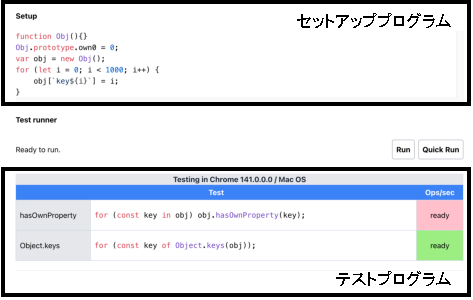
\includegraphics[width=1.0\linewidth]{./Noguchi_fig/jsPerf_example.pdf}
    \caption{マイクロベンチマーク共有サービスの投稿例\protect\footnotemark}
    \label{fig:jsPerf}
\end{figure}

\footnotetext{\url{https://jsperf.app/qiwudo}}
%----------------------

マイクロベンチマーク共有サービスは,開発者がプログラムの実行速度を比較・共有するためのオンラインサービスである.図\ref{fig:jsPerf}に,マイクロベンチマーク共有サービスの1つであるJsPerf上で実際に投稿されているマイクロベンチマークの例を示す.

マイクロベンチマーク共有サービスにおける各投稿は,1つのセットアッププログラムと,1つ以上のテストプログラムから構成される.図上部に示すセットアッププログラムでは,検証対象のコードで共通して利用される変数の初期化やデータの準備が行われる.一方,図下部に示すテストプログラムでは,同一の機能を異なる方法で実装したプログラム(大抵は短いソースコード片)が複数提示され,それぞれの実行速度を計測・比較できる.
このようなマイクロベンチマークは,データ構造や制御構文の選択,メソッド呼び出しの方法などに多様性が見られることが特徴であり,実行速度の差とその要因となる実装方法を捉えることができる.本研究では,このようなマイクロベンチマーク共有サービス上の実装対を分析し,性能効率性,特に実行速度に影響を与える構造的特徴を分析および抽出するために利用する.


% マイクロベンチマーク共有サービスの一つであるJsPerfにおいて,実際に投稿されているマイクロベンチマークの例を図\todo{スクショ挿入・リンクをフットノート}に示す,マイクロベンチマーク共有サービスでは,1つの検証における準備を行うセットアッププログラムと,検証対象となる2つ以上のテストプログラムから構成されている.図上部に示すプログラムがセットアッププログラムを示しており,検証対象のプログラムで利用される変数の初期化などが行われている.図下部に示すプログラムがテストプログラムを示しており,図では,\todo{コードの説明}と\todo{同じく}の実行速度が計測・比較検証される.

% マイクロベンチマーク共有サービスでは,図に示すような実装対が保存・公開されており,同一の機能を異なる方法で実装した非常に短いコードの対によって構成されており,データ構造や制御構文,使用するメソッドの選択などに多様性が見られる.


%2.2
\subsection{関連研究}

Selakovic ら\cite{jsRefac}は,JavaScriptを利用しているプロジェクトにおいて,開発者が高速化のために行ったリファクタリングを調査した.その結果,開発者は10行程度の小さい範囲の修正によって高速化への対処を行なっていることを明らかにした.この結果は,マイクロベンチマーク共有サービスに見られる,短いコードによる高速化への利用可能性を示すものとして,本研究の動機づけとなっている.また,\cite{jsRefac}は,JavaScript プロジェクトの解析によって 10 件の頻出する高速化改良パターンを作成している.この改良パターンを用いた自動修正は一定の高速化効果を示しているが,該当箇所の特定における制約などから,広範な適用には至っていない.

Turcotte ら\cite{DrAsync}は,JavaScript 言語における非同期処理に注目した性能アンチパターンを定義し,静的解析エンジンであるCodeQL\cite{ql}を利用したアンチパターンの検出と,動的解析を利用したパフォーマンスの監視を組み合わせ,修正可能な性能アンチパターンの検出を行った.本研究の静的解析による低速コードパターンの検出はこれに着想を得ている.

大森ら\cite{omori}は,マイクロベンチマーク共有サービスで公開される実行速度が向上するプログラムを収集し,これをデータセットとして大規模な言語学習モデルをファインチューニングすることで,実行を高速化するプログラムに自動リファクタリングするモデルを作成した.この結果,マイクロベンチマーク共有サービス上のプログラムに対しては,ChatGPT-4oより約3倍の件数の高速化リファクタリングに成功している.しかし,適用対象がマイクロベンチマーク共有サービス上のプログラムに留まっており,\cite{jsRefac}と同様,広範な適用には至っていない.

本研究では,繰り返し処理に注目し,マイクロベンチマーク共有サービスで公開される実装対における低速コードから,構造的差分に基づいて低速コードパターンを抽出し,静的解析を用いた性能ボトルネックの早期検出を行うとともに,適用範囲を拡張する上での検出精度の指標について議論する.\memo{あいまい...もっといい表現があるはず}


%%%%%%%%%%%%%%%%%%%%%%%%%%%
%3
\section{事前分析}
\label{sec:pre-analysis}
%%%%%%%%%%%%%%%%%%%%%%%%%%%


本研究では,大森ら\cite{omori}が作成した,マイクロベンチマーク共有サービスJsPerfにおける,実行速度に有意差があり,外的振る舞いが等しいことが検証された実装対29,809件を利用する.以降,この実装対をマイクロベンチマーク実装対とし,各実装対において,実行速度が遅いコードを低速コード,実行時間が速いコードを高速コードとする.

%3.1
\subsection{繰り返し処理を含むマイクロベンチマーク実装対}
\label{section3.1}

% \todo{図1で示すように} 繰り返し処理を含む実装対が全体の約43%(12,948対)存在する.

マイクロベンチマーク実装対を目視調査した結果,実装対の両方もしくは片方に繰り返し処理を含むものが多く存在することが確認された.特に,巨大な配列や長大な繰り返し処理を用いて性能差を強調する実装対や,繰り返し処理自体の違いによって実行時間に差が生まれる実装対など,複数の傾向が確認された.

このような観察結果から,本研究ではマイクロベンチマーク実装対に対して繰り返し処理構造に着目した特徴分析を行うこととした.対象とする繰り返し処理は,JavaScriptにおける for,for-of,for-in,while,および do-while 構文である.

分析にあたっては,各実装対のソースコードをGumTree\cite{gumtree}により抽象構文木へと変換し,実装対の抽象構文木間の差分解析を行った.差分解析の結果に対して,

(1) 差分が直接繰り返し処理構造を含むか

(2) 差分要素の構造的な親要素に繰り返し処理が含まれるか

を確認事項とし,繰り返し処理に関連する差分要素として収集した.抽出された箇所に応じて目視で確認を行い,実装対の構造的特徴および性能差との関係を整理した.
この分析の結果,マイクロベンチマーク実装対には繰り返し処理について,いくつかのパターンが存在することが明らかとなった.Listing~\ref{diff-loop},Listing~\ref{diff-inloop},Listing~\ref{diff-method}に,特徴となる部分について示す.

Listing~\ref{diff-loop}は,それぞれ,for-in文を用いて配列に含まれる要素にアクセスする実装と,同様の処理をfor文で実装したものである.ここで示すパターンは実行時間の差が,繰り返し処理自体の違いに起因するパターンである.
%----------------------------------
\begin{lstlisting}[caption=Pairs with loop differences, label=diff-loop, captionpos=t, columns=flexible]
// slow
for (key in VAR_1) {
    if (!VAR_1.hasOwnProperty(key)) continue;
    VAR_2 = VAR_1[key];
}

// fast
for (var VAR_8=0; VAR_8<VAR_1.length; ++VAR_8) {
    VAR_2 = VAR_1[VAR_8];
}
\end{lstlisting}
%----------------------------------

Listing~\ref{diff-inloop}は,それぞれfor文内で concat メソッド, push メソッドを用いている実装対である.これは,繰り返しの構造は一致しているが,繰り返し内部で実行する処理が異なるパターンである.
%----------------------------------
\begin{lstlisting}[caption=Pairs with differences within the loop, label=diff-inloop, captionpos=t, columns=flexible]
// slow
for (var VAR_2=0; VAR_2<5000; VAR_2++)
    VAR_1 = VAR_1.concat([\"1\", \"2\"]);

// fast
for (var VAR_2=0; VAR_2<5000; VAR_2++)
    VAR_1.push(\"1\", \"2\");
\end{lstlisting}
%----------------------------------

Listing~\ref{diff-method}は,繰り返し処理をforEachメソッドで実装したものとfor-of文で実装したものである.これは,メソッドによる処理とそれに代替する繰り返し処理について比較したパターンである.
%----------------------------------
\begin{lstlisting}[caption=Pairs of Method and alternative loop, label=diff-method, captionpos=t, columns=flexible]
// slow
var VAR_5 = new Set(VAR_2);
VAR_5.forEach(VAR_6 => {});

// fast
for (let VAR_7 of VAR_2) {}
\end{lstlisting}
%----------------------------------

これらの結果から,マイクロベンチマーク実装対には繰り返し処理の構造および繰り返し内部の操作内容の違いが性能差の要因の1つとして存在することが確認された.本研究では,このような繰り返し処理に関する差分構造を低速コードの特徴として抽出し,次章で述べる低速コードパターンの抽出および静的検出に利用する.


%%%%%%%%%%%%%%%%%%%%%%%%%%%
%4
\section{CodeQLクエリを用いた低速コードパターン検出手法}
\label{sec:approach}
%%%%%%%%%%%%%%%%%%%%%%%%%%%

%----------------------
\begin{figure*}[t]
    \centering
    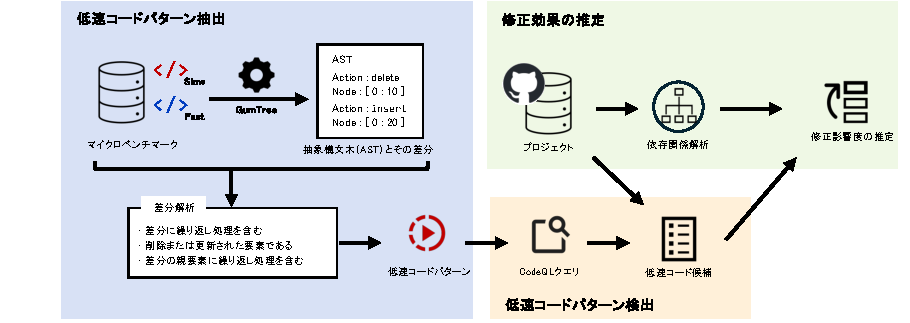
\includegraphics[width=1.0\linewidth]{./Noguchi_fig/approach_abst.pdf}
    \caption{手法概略図}
    \label{fig:Approach}
\end{figure*}
%----------------------

本研究では,実行速度の向上が期待されるソースコード片の検出に向けて,
マイクロベンチマーク共有サービスで提供される,実行速度の比較されたソースコード片の構造差分から低速コードパターンを作成する.これを利用し,静的解析エンジンCodeQLを用いて,ソースコード中から低速なソースコード片を検出する.図\ref{fig:Approach}は,本研究で提案する手法の概略図を示す.本手法は3つの方法で構成され,以降それぞれについて述べる.
% (1) マイクロベンチマーク実装対より,低速コードの特徴を実装対の構造的差分から抽出し,低速コードパターンを作成する.作成したパターンをもとに静的解析エンジンCodeQL\cite{ql}を用いて,ソースコード中の低速コードを静的に検出する手法を提案する.また,検出結果について,修正効果の高い箇所をプログラム中の依存関係の数から推定する.以降でその詳細を述べる.


%4.1
\subsection{分析対象ベンチマークの収集}

\ref{sec:pre-analysis}章で述べたように,著者らはマイクロベンチマーク共有サービスにおいて,繰り返し処理の構造および繰り返し内部の操作内容の違いが性能差の要因の1つであることを確認した.したがって,本研究では,差分解析を行い,従来研究で対象とするベンチマークの中で,比較されるソースコード間の差分に直接繰り返し処理構造を含む,または,差分要素の構造的な親要素に繰り返し処理が含まれるベンチマーク実装対を収集した.
% \memo{数を載せるか検討} 結果として29,806件の実装対から10,760対が対象となった.


%4.2
\subsection{低速コードのパターン作成}
本研究はベンチマークに含まれる低速コードから高速コードへの変更を仮定して,その構造的差分からパターンを作成する.差分抽出には,\ref{sec:pre-analysis}章同様,GumTreeを使用し,差分要素とその変更操作を取得した.

GumTree によって得られた構造的差分および変更操作のうち,低速コードから削除または更新された要素を抽出する.これらの要素は,高速コードに存在しない要素であり,低速コード特有の処理や構造を示す要素であると考えられるため,低速コードの特徴候補として収集する.Listing~\ref{diff-loop}に示す実装対にこの処理を行うと,Listing\ref{candidates}における,背景色のついた要素が低速コードの特徴候補として収集される.

次に,収集した低速コードの特徴候補から,繰り返し処理および繰り返し処理の条件,メソッド呼び出し,配列・オブジェクト操作を,意味的に有効な要素として抽出する.それぞれの要素について,低速コードにおける開始位置および終了位置や階層情報を参照し,抽出した要素を統合することで,低速コードパターンを形成する.この操作によって,複数の実装対に共通して出現する低速コード特有の構文的特徴を捉える.

以上の処理を行うことで,Listing~\ref{diff-loop}では,図\ref{fig:slow_pattern}に示すような,「if文に .hasOwnProperty() 呼び出しを持つ for-in 文」というパターンが生成される.

%----------------------------------
\begin{lstlisting}[caption=Characteristic Candidates for Slow Code, label=candidates, captionpos=t, columns=flexible, literate=
    {for}{{\textcolor{black}{\colorbox{lightred}{for}}}}{3}
    {key}{{\textcolor{black}{\colorbox{lightred}{key}}}}{3}
    {in }{{\textcolor{black}{\colorbox{lightred}{in}}\kern0.5em}}{3}
    {VAR\_1}{{\textcolor{black}{\colorbox{lightred}{VAR\_1}}}}{5}
    {if}{{\textcolor{black}{\colorbox{lightred}{if}}}}{2}
    {!}{{\textcolor{black}{\colorbox{lightred}{!}}}}{1}
    {hasOwnProperty}{{\textcolor{black}{\colorbox{lightred}{hasOwnProperty}}}}{15}
    {continue}{{\textcolor{black}{\colorbox{lightred}{continue}}}}{8}
    {VAR\_1\_}{{\textcolor{black}{VAR\_1}}}{6}
]
for (key in VAR_1) {
  if(! VAR_1.hasOwnProperty(key))continue;
  VAR_2 = VAR_1_[key];
}
\end{lstlisting}
%----------------------------------

%----------------------
\begin{figure}[!h]
    \centering
    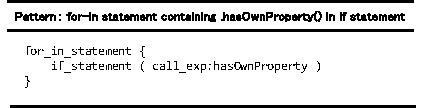
\includegraphics[width=1.0\linewidth]{./Noguchi_fig/slow_pattern.pdf}
    \caption{低速コードパターン例}
    \label{fig:slow_pattern}
\end{figure}
%----------------------



%4.3
\subsection{低速コードパターンの検出}

本研究では,作成した低速コードパターンに基づく検索クエリを作成し,静的解析ツールCodeQL\cite{ql}を用いて低速なソースコード片を検出する.CodeQLは,GitHubが主にセキュリティ検査を自動化する目的で開発されたコード分析ツールである.具体的には,分析対象とするプログラムから抽象構文木,データフロー情報,型情報,呼び出し関係などをデータベースに保持する.このデータベースに対して,SQLに似たクエリ言語を用いて,特定の構造や振る舞いを持つソースコード検索を実現している.
本研究では,低速コードパターンをもとにCodeQLに対応するクエリを作成し,ソースコード内で同様の構造を持つ箇所を検出する.


%%%%%%%%%%%%%%%%%%%%%%%%%%%
%5
\section{評価方法\todo{ここは結果を見てから直す}}
\label{sec:evaluation}
%%%%%%%%%%%%%%%%%%%%%%%%%%%

本研究では,提案手法の有効性を検証するために,低速コードパターンを含むソースコードの検出を行い,検出結果に対し,パターンの元となった低速コードとの類似度から検出の妥当性について評価を行う.

類似度はCode2Vec\cite{code2vec}を用いてソースコード片を分散表現化し,コサイン類似度を用いて算出する.なお,Code2Vecは,\cite{saiki}より,JavaScriptに対応したパスコンテキスト変換処理と学習モデルを利用した.

% パターンの元となった低速コードと類似度の高いソースコード片上位\todo{n}件とを選択し,低速コードパターンの元となった実装対との類似度を算出する.次に,目視により各検出箇所が,クエリの元となったマイクロベンチマーク実装対における低速コードの特徴を正しく捉えているかを確認する.
% 各類似度指標と目視確認結果と照らし合わせることで,どの指標・閾値設定が低速コード検出に最も有効であるかを議論する.


\ihara{ここまで修正済み}

%%%%%%%%%%%%%%%%%%%%%%%%%%%
%6
\section{ケーススタディ}
\label{sec:case-study}
%%%%%%%%%%%%%%%%%%%%%%%%%%%

ケーススタディとして,提案手法によって作成された低速コードパターン6件について,CodeQLクエリを作成し,CodeQLを用いて低速コードパターンを含むソースコード片の検出を行う.利用する低速コードパターンを表\ref{tab:slow_code_patterns}に示す.\todo{全部見せるかは検討}
なお,CodeQLクエリの作成では,作成したクエリをマイクロベンチマーク実装対に適用し,元となった低速コードパターンを含むソースコード片を検出できるか,および,対象となる低速コードパターンを含まないソースコード片を検出しないかを目視で確認し,クエリの妥当性を検証した.

%----------------------
\begin{table}[h!]
    \centering
    \caption{低速コードパターン}
    \label{tab:slow_code_patterns}
    \setcounter{patternID}{0} % 表が始まる前にカウンタを0にリセット
    \resizebox{1.0\linewidth}{!}{
        \begin{threeparttable}
            \begin{tabular}{clr}
                \toprule
                \textbf{ID} & \textbf{特徴} & \textbf{該当数\tnote{*}} \\
                \midrule
                
                \refstepcounter{patternID}\label{ptn:for-in}
                \thepatternID & for-in文 & 351 \\
                
                \refstepcounter{patternID}\label{ptn:forEach}
                \thepatternID & .forEach()呼び出し & 328 \\
                
                \refstepcounter{patternID}\label{ptn:hasOwnProperty}
                \thepatternID & if文に.hasOwnProperty()呼び出しを持つfor-in文 & 78 \\
                
                \refstepcounter{patternID}\label{ptn:json}
                \thepatternID & .parse(.stringify())呼び出し & 27 \\
                
                \refstepcounter{patternID}\label{ptn:applymap}
                \thepatternID & .apply().map()呼び出し & 11 \\
                
                \refstepcounter{patternID}\label{ptn:push}
                \thepatternID & .push()呼び出しを持つfor-of文 & 10 \\
                \bottomrule
            \end{tabular}
            
            \begin{tablenotes}
                \raggedleft
                \item[*] そのパターンに該当するマイクロベンチマーク実装対の数
            \end{tablenotes}
        \end{threeparttable}
    }
\end{table}
%----------------------

%6.1
\subsection{データセット}

低速コードパターン検出における対象データセットとして,プログラムバージョン管理システムであるGitHubで公開されている,主要言語がJavaScript,最終コミットが1年以内のプロジェクトより,スター数上位1,000プロジェクトを選定した.

%6.2
\subsection{低速コードパターンの検出}

表\ref{tab:result_detect}は,表\ref{tab:slow_code_patterns}に示した各低速コードパターンの検出結果を示したものである.左の列から,パターンID,検出数が0より大きいプロジェクト数,単一プロジェクトにおける最大検出数,1,000プロジェクトにおける総検出数を示す.また,図\ref{fig:plot_id3}は,そのうち,ID \ref{ptn:hasOwnProperty}について,各プロジェクトの規模(JavaScriptファイルの行数)と,各プロジェクトで検出された低速コードパターンの数についての分布を示したものである.各点はデータセット中の各プロジェクトを示している.

%----------------------
\begin{table}[h!]
    \centering
    \caption{検出結果}
    \label{tab:result_detect}
    \resizebox{1.0\linewidth}{!}{
        \begin{tabular}{crrr}
            \toprule
            \textbf{ID} & \textbf{検出数 \texttt{>} 0 (プロジェクト)} & \textbf{最大検出数 (件)} & \textbf{総検出数 (件)} \\
            \midrule           
            \ref{ptn:for-in} & 689 & 7378 & 90592 \\
            \ref{ptn:forEach} & 842 & 12675 & 161681 \\
            \ref{ptn:hasOwnProperty} & 308 & 1125 & 9516 \\
            \ref{ptn:json} & 282 & 142 & 2684 \\
            \ref{ptn:applymap} & 48 & 12 & 138 \\
            \ref{ptn:push} & 477 & 3351 & 30075 \\
            \bottomrule
        \end{tabular}
    }
\end{table}
%----------------------

%----------------------
\begin{figure}[h!]
    \centering
    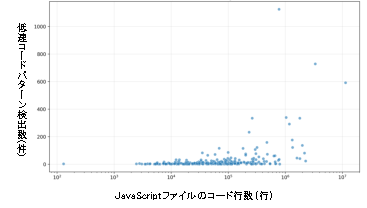
\includegraphics[width=0.9\linewidth]{./Noguchi_fig/ID3_222_log.pdf}
    \caption{低速コードパターンID3による検出数と規模}
    \label{fig:plot_id3}
\end{figure}
%----------------------


表\ref{tab:result_detect}で示すように,低速コードパターンは48から842プロジェクトで検出され,パターンごとに検出数の差異が見られたものの,利用したすべての低速コードパターンにおいて,実際にマイクロベンチマークに存在した構造と一致する検出結果が得られた.また,表\ref{tab:slow_code_patterns}におけるID\ref{ptn:for-in}や,ID\ref{ptn:forEach}の低速コードパターンのように,マイクロベンチマーク実装対における該当数が多いパターンは実プロジェクトにおいても検出数が多くなった.

加えて,図\ref{fig:plot_id3}で示すように,プロジェクト規模が大きくなるほど低速コードパターンの検出数が多くなる傾向が見られた.なお,他の低速コードパターンによる検出結果についても同様の傾向が見られた.
\memo{プロジェクト別に検出数とか特徴に関係があるかを追加で見る必要あり}


%6.3
\subsection{検出結果の類似度}\todo{目視の実例入れてもいいかも}

次に,1つのパターンについて,検出されたコード片から,Code2Vecを用いて分散表現を取得し,低速コードパターンの元となったマイクロベンチマーク実装対における低速コード群とコサイン類似度を計測する.対象パターンをID \ref{ptn:hasOwnProperty}とし,パターンの元となった低速コードとのコサイン類似度の平均値について図\ref{fig:boxplot_cosine}に示す\memo{具体的な数を言う?}.なお,比較対象として,マイクロベンチマーク実装対における低速コードに対し,CodeQLを用いて低速コードパターン検出を行い,結果について同様の処理を行った結果を図\ref{fig:boxplot_cosine}の右側に示している.

% ベクトル化したのは,7039/9516件 

%----------------------
\begin{figure}[h!]
    \centering
    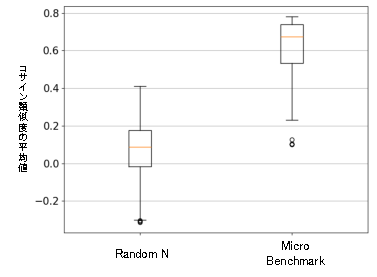
\includegraphics[width=0.9\linewidth]{./Noguchi_fig/boxplot_compare.pdf}
    \caption{検出結果とパターン元低速コードのコサイン類似度\todo{ラベル差し替え}}
    \label{fig:boxplot_cosine}
\end{figure}
%----------------------

実プロジェクトにおける検出結果では,平均値0.08,中央値0.09,マイクロベンチマーク実装対では,検出件数123件について,平均値0.61,中央値0.68となった.

\memo{マイクロベンチマークとの比較をする.規模感・変数名の近さで高くなっていることは考察?}
それぞれの結果について,目視でコサイン類似度とソースコード片を確認したところ\memo{上位10・第1〜第3四分位数のそれぞれ10・下位10の計50個を目視.載せるか&目視増やすか&見る箇所変えるかは検討},コサイン類似度の高低に関わらず,作成したクエリが示す低速コードパターンを含んでいることを確認した.一方で類似度の高いソースコード片については,マイクロベンチマーク実装対における低速コードと,コード長および構造が類似するコード片や,変数名が短く単純なコード片が多く見られた.類似度が低いソースコード片では,全体のコード長が大きいものや,変数名が長い,リテラルを多く含むコードが多く見られた.


%%%%%%%%%%%%%%%%%%%%%%%%%%%
%7
\section{考察}
\label{sec:discussion}
%%%%%%%%%%%%%%%%%%%%%%%%%%%


%7.1
\subsection{検出結果}

提案手法により作成した低速コードパターンは,実際のソースコード中から検出されたことから,提案手法によって,マイクロベンチマーク実装対をもとに抽出した構造差分が,現実のプログラムにおける処理構造を捉えることができたと考えられる.なお,プロジェクト規模が大きいほど検出数が増加した点については,コード量の増大に伴って低速コードパターンに該当するコード片が出現する確率が増加することが反映されており,妥当であると言える.

一方で,低速コードパターンの検出数が多い場合,そのパターンが広く利用されていることを示すが,必ずしもすべてが修正対象として優先されるわけではない.
したがって,修正効果の大きい箇所を抽出して示す必要がある.今後の課題として,検出結果について,関数間の依存関係やデータフロー構造といったものを考慮し,修正が性能全体に与える影響を推定する仕組みを構築することが挙げられる.

%7.2
\subsection{類似度指標\memo{もっと深められるはず...}}

検出結果に対する,コサイン類似度による評価と目視分析の結果から,CodeQLにより検出されたコード片は,低速コードパターンを含んでおり,作成したクエリが構造的に妥当であることが確認された.これは,CodeQLが抽象構文木に基づき構造的特徴を正確に抽出できていることを意味し,構文的な類似度はこの段階で一定程度確保できていると考えられる.

一方で,コサイン類似度に目視で確認した構造的特徴の類似が大きく反映されることは確認できなかった.これは,Code2Vecによるベクトル化において,コード長や変数名の情報が類似度計算に強く影響していることが考えられる.特に,マイクロベンチマーク実装対が短いコード片であることから,長大なコードや変数名の多様性を持つ実プロジェクトでは,構造的類似度と意味的類似度が十分に反映されない可能性が示唆される.この点については,変数名の抽象化や,JavaScriptコードに特化した学習モデルの再構築によって改善が期待される.

なお,現時点で類似度が高い検出結果については,コード長が短く,また,低速コードパターンの元となった低速コードの構造に類似しているものであったことから,マイクロベンチマークを参照した修正が比較的容易に適用できる可能性を示している.したがって,検出結果に対するコサイン類似度を用いた評価は,性能改善の容易性を示す指標として有用である可能性が示唆される.
\memo{体感0.2ぐらいの類似度が規模感の近さと修正できそう感の閾値.0.1を下回ると目視しんどいレベルのサイズが増える}


\subsection{妥当性の脅威}

%7.3
\noindent\textbf{内的妥当性: }
本研究では,低速コードの特徴抽出をGumTreeによる差分解析に依存している.したがって,抽出された差分が必ずしも低速コードの特徴を正確に表現していない可能性が存在する.本研究では,差分から得られた要素を目視により確認し,実装例と照合した上でパターンを作成しているため,その影響は小さいと考えるが,今後パターン数を拡張する際には,差分抽出の精度や作成手法の改善が課題となる.

また,低速コードパターンの検出におけるパターンのクエリ化を,GumTreeによる差分解析結果をもとに手作業で行っている.そのため,作成したクエリが低速コードパターンを正確に反映しているかについては,目視による確認に依存しており,一定の主観的判断が含まれる可能性がある.ただし,本研究では,マイクロベンチマークに対して実際にクエリを適用し,想定した低速ソースコード片が検出されることを確認しており,その影響は限定的であると考える.

本研究で利用したマイクロベンチマーク共有サービスであるJsPerfは2020年にサービスを終了しており,当時の高速実装が現在においても最適であるとは限らない.この点については,関連研究\cite{omori}においても同様の指摘がなされている.

本研究における類似度計測においては,プログラム断片のベクトル化にCode2Vecを利用している.本来の Code2VecはJavaおよびC\#を対象としているため,それらの言語への利用における精度と差異が生じる可能性がある.本研究ではJavaScript対応かつマイクロベンチマークをもとに学習された学習モデル\cite{saiki}を使用することで,この影響を抑えるよう努めた.

\noindent\textbf{外的妥当性: }
本研究におけるケーススタディでは,時間的制約のため,GitHub上のスター数上位のプロジェクトに対象を限定して分析を行った.そのため,結果の一般性は限定的である可能性がある.
特にスター数の多いプロジェクトは,既に十分に最適化・保守が行われていることが多いため,このようなプロジェクトにおける検出結果は,一般的な開発段階のソフトウェアとは異なる可能性がある.

また,本研究では,低速コードパターンを6個作成し,ケーススタディを実施し,類似度計測ではそのうち1つのパターンについての検証となっている.異なるパターンに対しては,同様の手法で実験を行う必要があり,複数パターンに基づく評価によって,提案手法の汎用性および有効性をさらに検証することが今後の課題である.


%%%%%%%%%%%%%%%%%%%%%%%%%%%
%7
\section{おわりに}
\label{sec:summary}
%%%%%%%%%%%%%%%%%%%%%%%%%%%

本研究では,ソフトウェア中に潜在する,修正によって実行速度の向上が期待されるソースコード片を検出することを目的とし,マイクロベンチマーク共有サービスで提供されるベンチマーク実装対の構造差分から低速コードパターンを抽出し,静的解析エンジンであるCodeQLを用いて実際のソースコード中から低速コードを検出する手法を提案した.

ケーススタディとして,6件の低速コードパターンおよび,それぞれに対応するCodeQLクエリを作成し,GitHub上の実プロジェクト1,000件を対象に検出実験を行った.その結果,提案手法によって作成した低速コードパターンが実際のソースコード中から検出され,マイクロベンチマーク共有サービス由来の構造差分が,実際のプログラムにおける処理構造を適切に捉えられていることを確認した.

さらに,検出結果に対してCode2Vecを用いたベクトル化を行い,コサイン類似度による評価および目視分析を実施した結果,CodeQLによって検出されたコード片はいずれも低速コードパターンを含んでおり,作成したクエリが構造的に妥当であることを確認した.これは,CodeQLが抽象構文木に基づいて構造的特徴を正確に抽出できていることを示唆している.一方で,コサイン類似度は構文的な類似性よりも,コードの長さや変数名などの表層的特徴に強く影響される傾向が見られた.特に,マイクロベンチマークが短いコード片で構成されていることから,より複雑な構造や多様な変数名を含む検出結果に対しては,構文的および意味的類似度が十分に反映されない可能性が示唆された.

今後の課題としては,差分抽出やパターン生成,クエリ作成のさらなる自動化・拡張を進め,手法の再現性と汎用性を高めることが挙げられる.また,コサイン類似度以外のモデルや評価指標の検討を通じて,より意味的な類似性を捉えられる指標の構築を目指す.さらに,検出後の修正影響範囲を明らかにするために,依存関係解析などを組み合わせることで,より実践的な性能改善支援手法へ発展させることを今後の展望とする.

\begin{acknowledgment}
本研究はJSPS科研費 25K15058の助成を受けたものである.
\end{acknowledgment}



\bibliographystyle{ipsjunsrt}
\bibliography{bibnoguchi}

\end{document}
